\documentclass{article}
\usepackage[utf8]{inputenc}
\usepackage[hidelinks]{hyperref}
\usepackage{amsmath}
\usepackage[noabbrev, capitalise]{cleveref}
\usepackage{amssymb}
\usepackage{graphicx}
\usepackage{float}
\usepackage{subfig}
\usepackage{booktabs}
\usepackage[parfill]{parskip}

\usepackage[sorting=none]{biblatex}
\addbibresource{report_1.bib}

\usepackage{titling}
\setlength{\droptitle}{-3cm}

\title{COMP6247 Lab 1: Recursive Least Squares}
\author{Wei Chien Teoh (Eugene)\\\bigskip \href{mailto:wct1c16@soton.ac.uk}{wct1c16@soton.ac.uk}}
\date{22 February 2021}

\begin{document}

\maketitle

\section{Introduction}

This report presents to findings and results for Lab 1 of COMP6247 of University of Southampton \cite{lab1}. The code implementation is stored in a Github repository \cite{github}.

\section{Task 1} \label{section:task-1}

The task 1 of the exercise is to implement a simple linear regression on synthetic data solved with three different methods, namely: (i) closed form (pseudo-inverse); (ii) gradient descent (GD); (iii) stochastic gradient descent (SGD). The synthetic data generated involves a design matrix $X \in \mathbb{R}^{N \times p}$ and a set of weights $w_* \in \mathbb{R}^p$. In this example, $N$ (number of sample) and $p$ (number of features) are set to 500 and 30 respectively. The data is generated from a gaussian distribution $X, w_* \sim \mathcal{N}(0.5, 1)$ using Numpy. The target data $y$ is defined as the product $Xw_*$ added with noise also sampled from a gaussian distribution $\mathcal{N}(0, 1)$.

\cref{fig:lr_closed} shows the predicted results against the true values of targets and weights. Although the variance of the plots are large, there exist a linear relationship between true values and the prediction. This means that the closed form solution successfully provided a solution for the linear regression. The result plots for GD and SGD are very similar to that of \cref{fig:lr_closed}, hence they will be excluded in this report. The linear relationship is better represented as pearson correlation, shown in \cref{tab:task1_corr}.

\begin{figure}[h!]
    \centering
    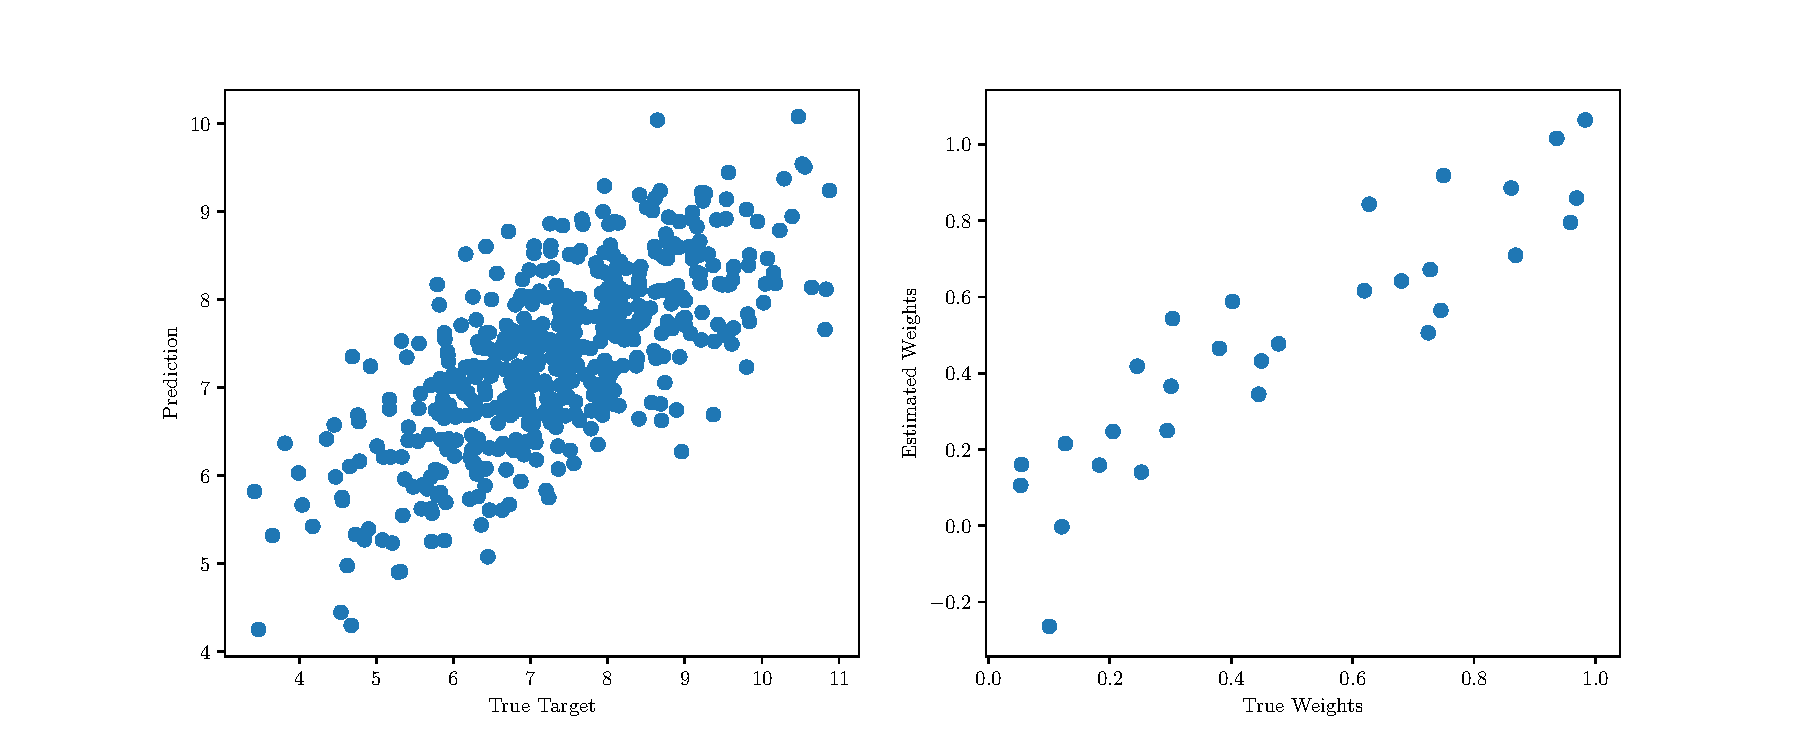
\includegraphics[width=\textwidth]{Figures/closed.pdf}
    \caption{Results of Linear Regression estimated with closed form. (Left) true value of target against prediction. (Right) true values of weights against estimated weights.}
    \label{fig:lr_closed}
\end{figure}

Pearson correlation shows the strength of linear correlation. A strong linear correlation shows that the predicted values are close to the ground truth. All three methods show promising and very close results. Thus, it can be concluded that all three methods successfully estimated the linear regression. Out of the three, the closed form solution performed the best.

The loss function of linear regression is always convex, hence there exist a closed form solution. However, if the number of features $p$ is large, the pseudo-inverse may be expensive to compute. The time complexity of matrix inversion (using Gaussian elimination) is $\mathcal{O}(n^3)$, hence it does not scale well with larger matrices.

\begin{table}[h!]
    \centering
    \caption{Table of correlation against ground truth on synthetic data.}
    \label{tab:task1_corr}
    \begin{tabular}{lrr}
    \toprule
    {} &         y &         w \\
    \midrule
    Ground Truth &  1.000000 &  1.000000 \\
    Closed Form  &  0.704550 &  0.901110 \\
    GD           &  0.704451 &  0.901576 \\
    SGD          &  0.697499 &  0.852364 \\
    MBGD         &  0.704231 &  0.895733 \\
    RLS          &  0.704521 &  0.901942 \\
    \bottomrule
    \end{tabular}
    
\end{table}
    
    
    

\cref{fig:gd_training} shows the training error against the number of iterations for two variants of gradient descent, batch and stochastic. \cref{fig:gd} shows the batch gradient descent training with the learning rate set to $10^{-4}$ for 500 iterations. \cref{fig:sgd} shows the stochastic gradient descent training with learning rate set to 0.005 for 5000 iterations.

With batch gradient descent, it requires less iterations than stochastic gradient descent to achieve the convergence of the loss function. It also shows a smoother convergence with less fluctuation of error. However, as the number of data samples $N$ gets larger, the derivative of the loss function with respect to the weights, $\nabla_{\boldsymbol{w}} E$ will be more expensive to compute.

Stochastic gradient descent was proposed to provide a scalable solution with large $N$. \cref{fig:sgd} show the training error across the number of iterations. SGD provides similar performance to batch gradient descent, but with much more fluctuation. If the training is stopped at a training iteration with high fluctuation, it will cause the error at that iteration to be large. \cref{fig:sgd_noise} shows a visual intuition of gradient descent updates close the convergence of loss function. The fluctuations of \cref{fig:sgd} are caused by oscillations between the valley of the convex loss function.

\begin{figure}[h!]
    \subfloat[Batch Training]{\label{fig:gd}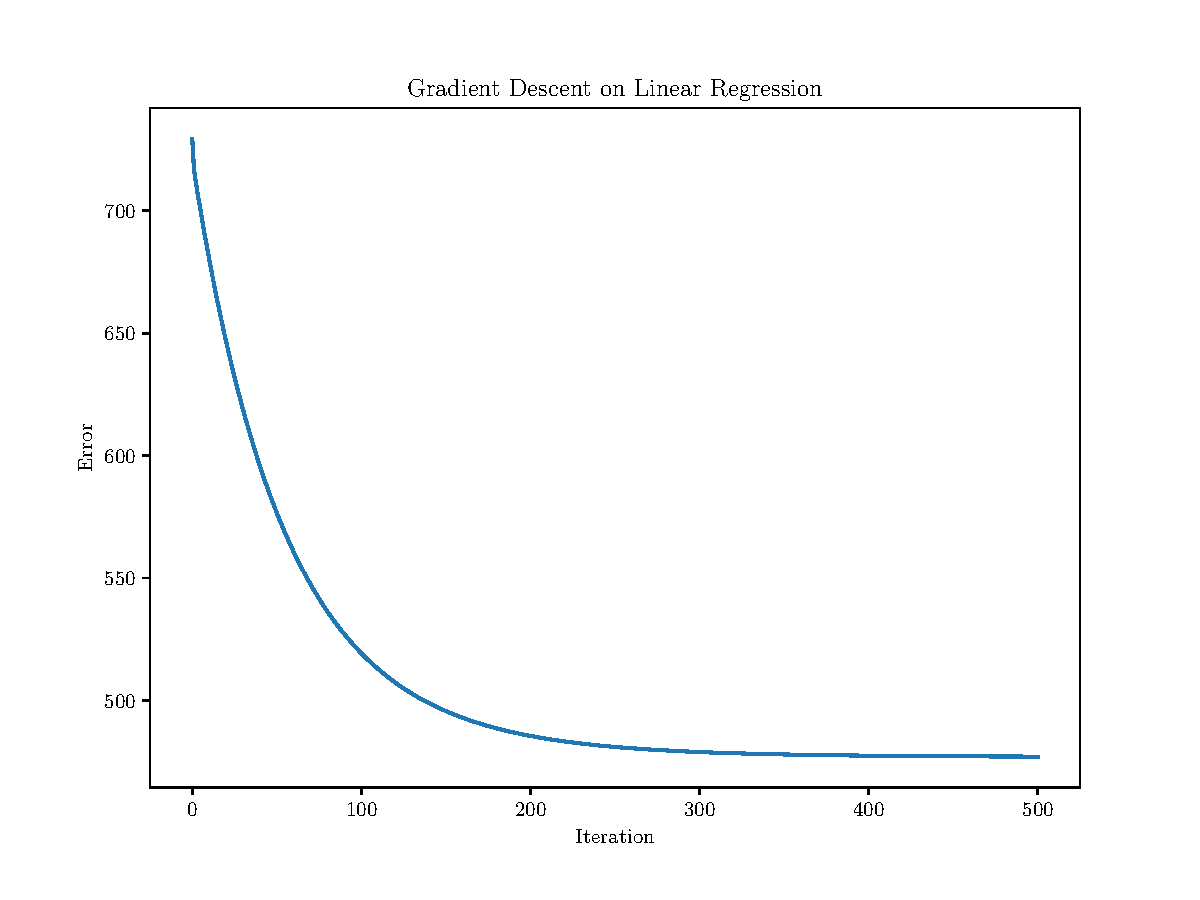
\includegraphics[width=0.33\textwidth]{Figures/gd_iterError.pdf}}
    \subfloat[Stochastic Training]{\label{fig:sgd}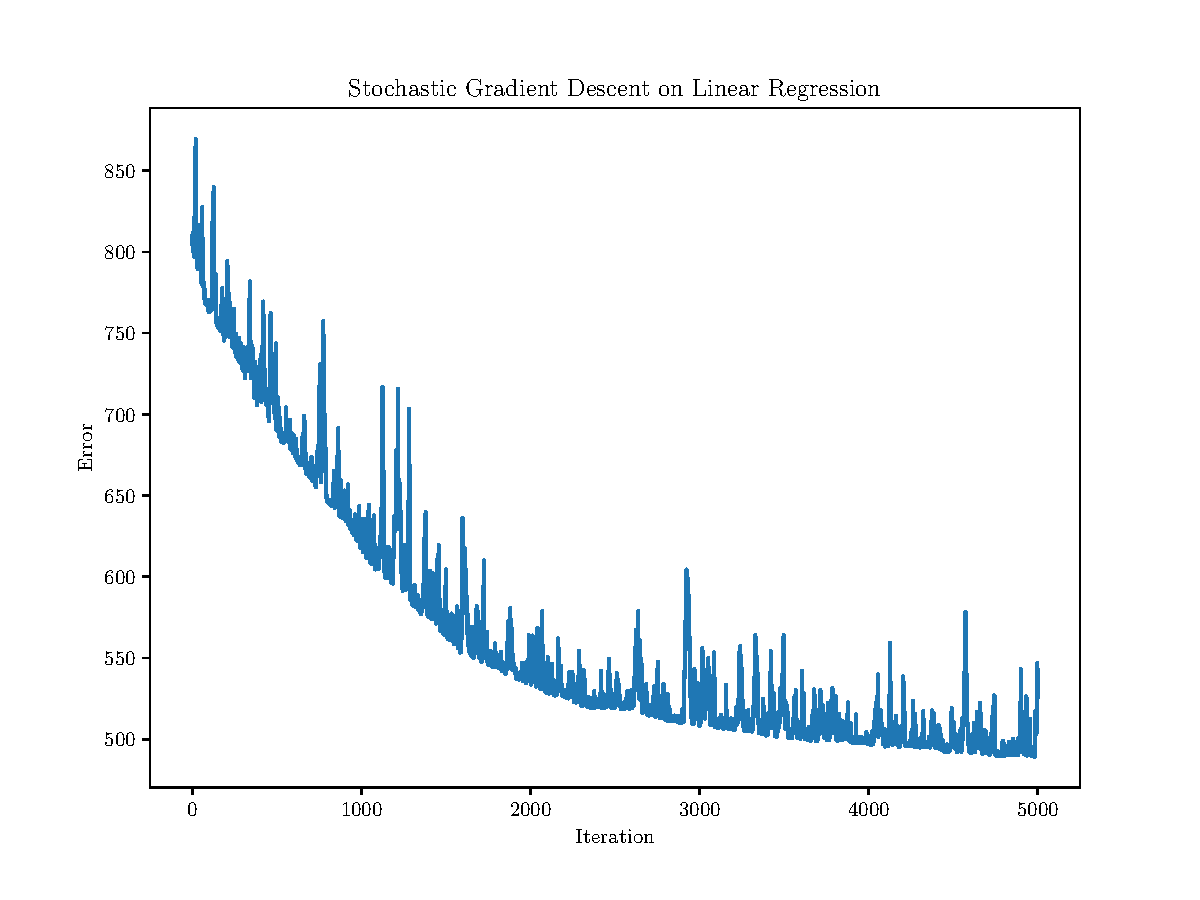
\includegraphics[width=0.33\textwidth]{Figures/sgd_iterError.pdf}}
    \subfloat[Mini-batch Training]{\label{fig:mbgd}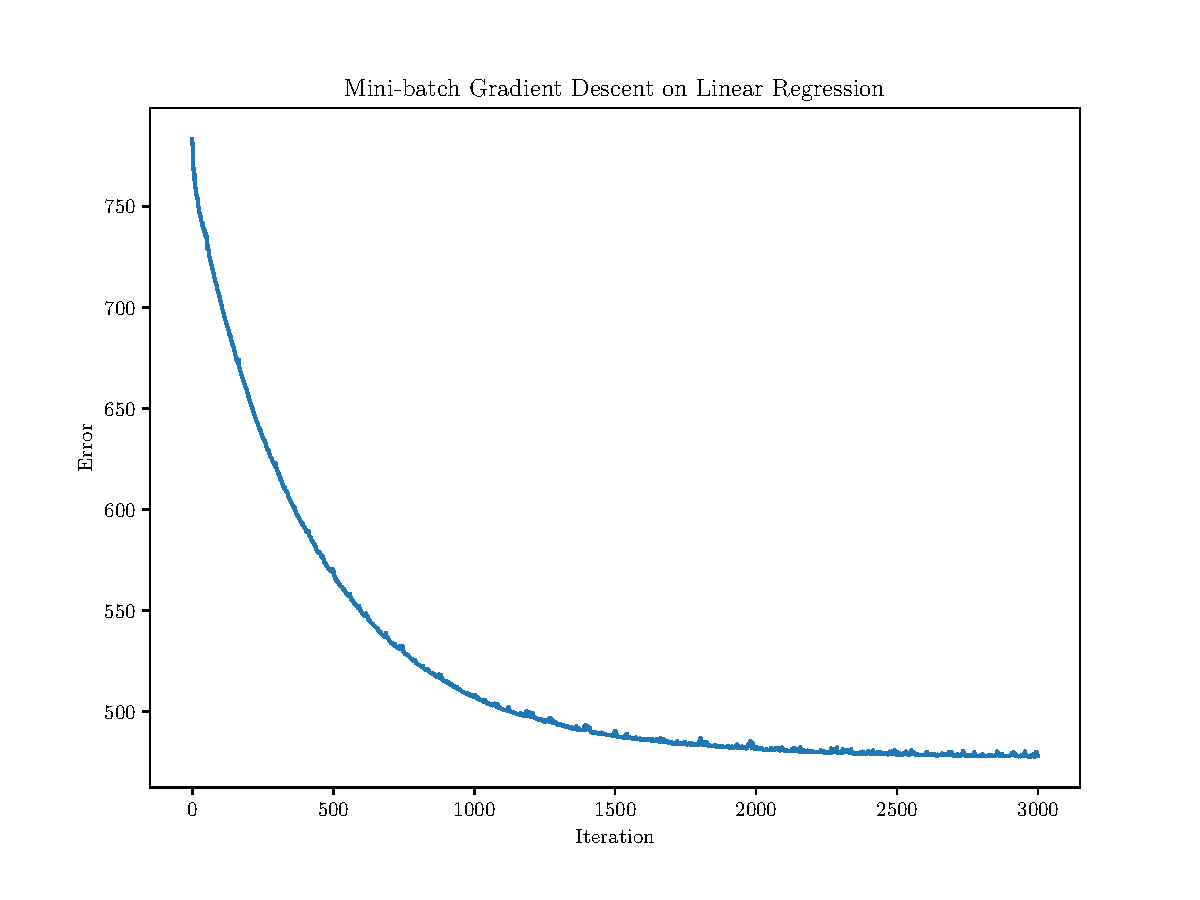
\includegraphics[width=0.33\textwidth]{Figures/mbgd_iterError.pdf}}
    \caption{Gradient Descent Training of Linear Regression.}
    \label{fig:gd_training}
\end{figure}

\begin{figure}[h!]
    \centering
    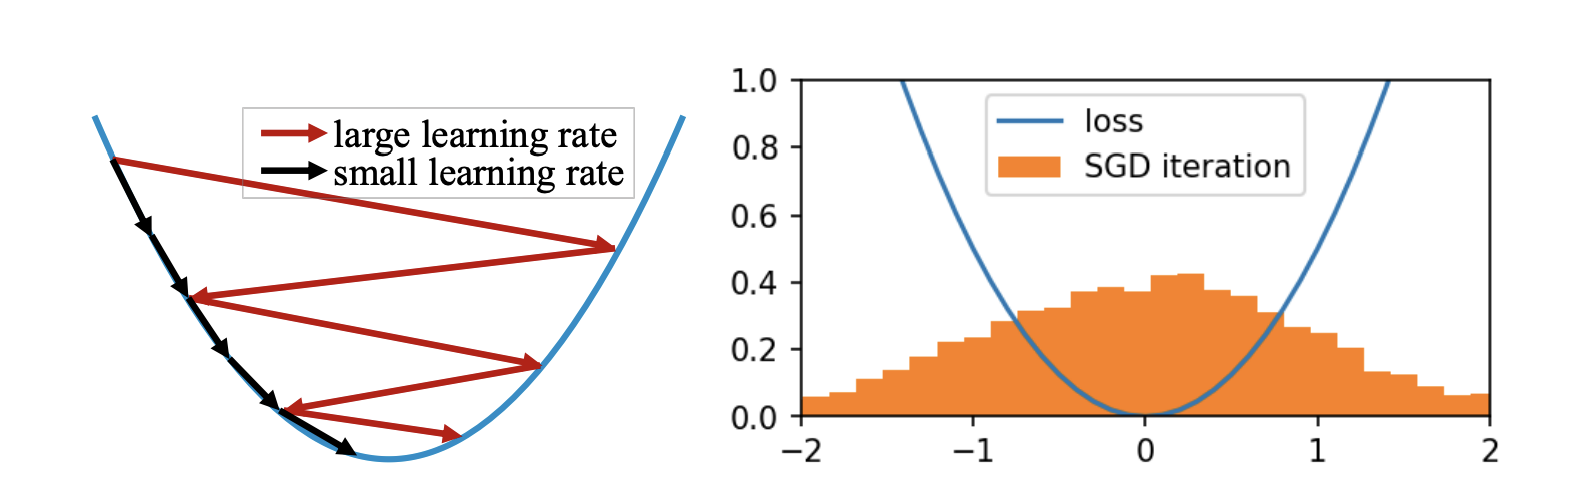
\includegraphics[width=0.8\textwidth]{Figures/sgd_update.png} 
    \caption{(Left) Effects of magnitude of learning rate on gradient descent update. (Right) Distribution of SGD loss convergence. (Sourced from \cite{liu2021noise})}
    \label{fig:sgd_noise}
\end{figure}

Mini-batch gradient descent (MBGD) is a variant of SGD, where instead of updating the weights based on one data sample, it uses a small batch of data. \cref{fig:mbgd} shows an implementation of MBGD with learning rate, iterations and batch size of $10^{-4}$, 3000 and 64, respectively. MBGD captures the best aspects of both GD and SGD. It allows faster updates by using a small subset of data sample, as well as preventing fluctuations of error.


\section{Task 2}

Recursive least squares (RLS) was implemented by myself on the synthetic data used in \cref{section:task-1}. \cref{fig:rls} shows the absolute error against the number of iterations for three different values of $p$. The plot shows some fluctuation of error during convergence. This is due to to the variance of the synthetic data generated. As RLS updates the weights one data point at a time, if the data point differs from the mean by a large amount, the error will also be large, thus causing the weights to update according to the error, hence the fluctuations. From the plot, it is shown that the error converges around the same number of iterations even as $p$ increases. Hence, we can also conclude that the speed of convergence does not increase with the dimensionality of the problem.

\cref{tab:task1_corr} includes the pearson correlation of RLS against the true target and weights. The performance shown is very promising, similar to the other methods described above. However, RLS is more flexible as it can be used in an online setting, where new data is received on new time steps. Thus it can be concluded that the RLS is correctly implemented.

\begin{figure}[h!]
    \centering
    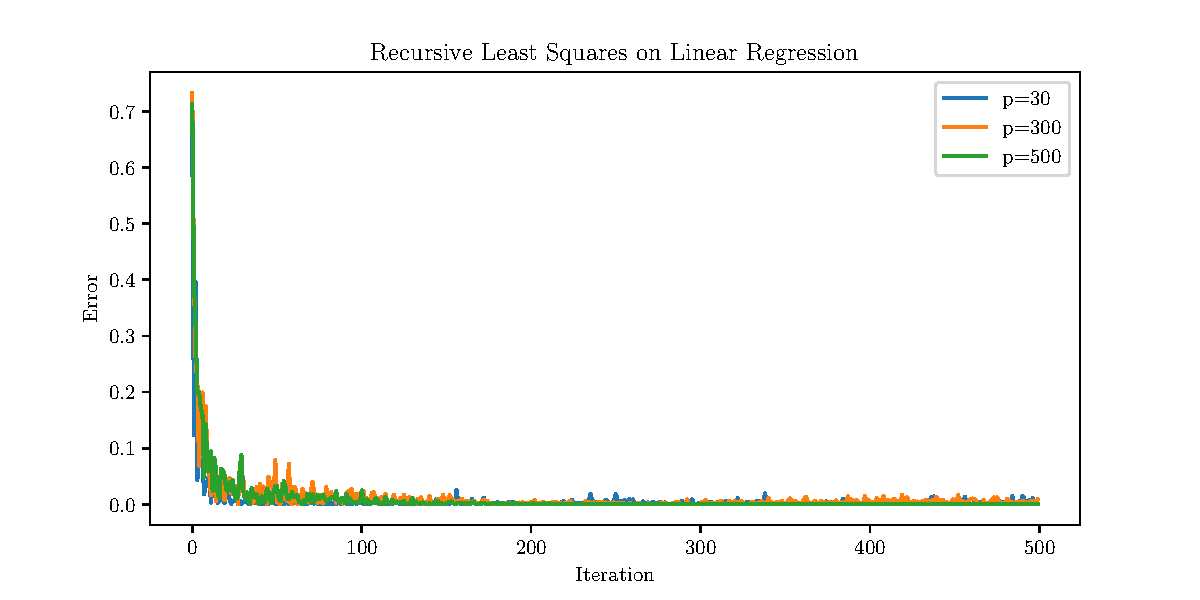
\includegraphics[width=0.8\textwidth]{Figures/rls_iterError.pdf}
    \caption{Recursive least squares absolute error.}
    \label{fig:rls}
\end{figure}

% TODO: Is there a trend/relationship between the speed of convergence and the dimensionality of the problem?

\section{Task 3}

In this task, the Computer Hardware Data Set from UCI Machine Learning Repository is used \cite{uci_dataset}. The features (or columns) in the design matrix $X$ are standardised with z-score.

\cref{fig:uci_sgd} shows the training plot of the Computer Hardware Dataset using SGD. Learning rate and number of iterations of $10^{-3}$ and 5000 is used for training. The plot shows a relatively smooth curve as compared to \cref{fig:sgd}. This is likely due to a smaller variance in the dataset.

\cref{fig:uci_rls} shows the training plot of squared error using RLS. The forgetting factor $\lambda$ is set to 0.98. The plot shows much fluctuation likely due to variance of the data. Although fluctuation exist, \cref{tab:task3_corr} shows that the predicted target performance using RLS is similar to the SGD method.

As RLS assumes one sample of data is received at a time, it is more prone to variance of data. Therefore, SGD is shown to provide better performance in this case.

\begin{figure}[h!]
    \subfloat[SGD]{\label{fig:uci_sgd}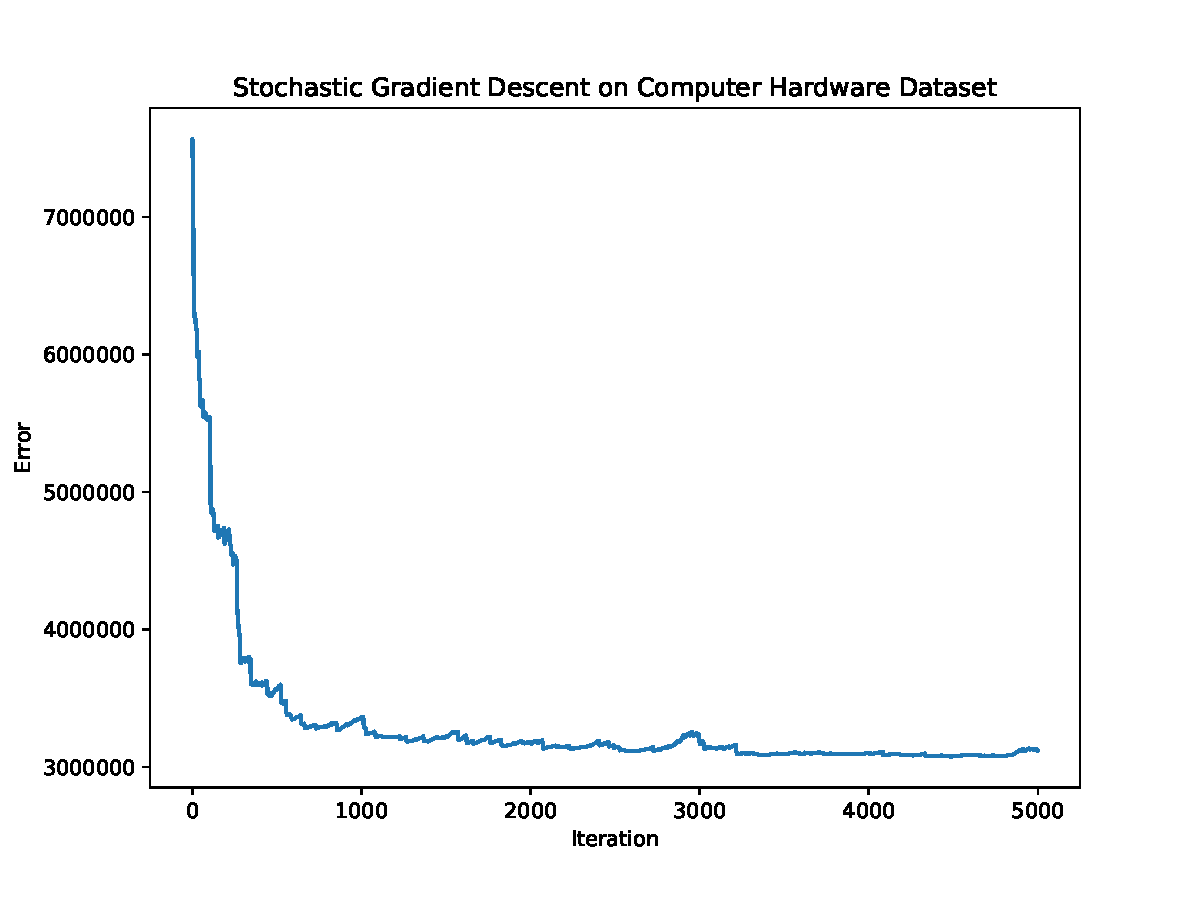
\includegraphics[width=0.33\textwidth]{Figures/uci_sgd_iterError.pdf}}
    \subfloat[RLS with own implementation]{\label{fig:uci_rls}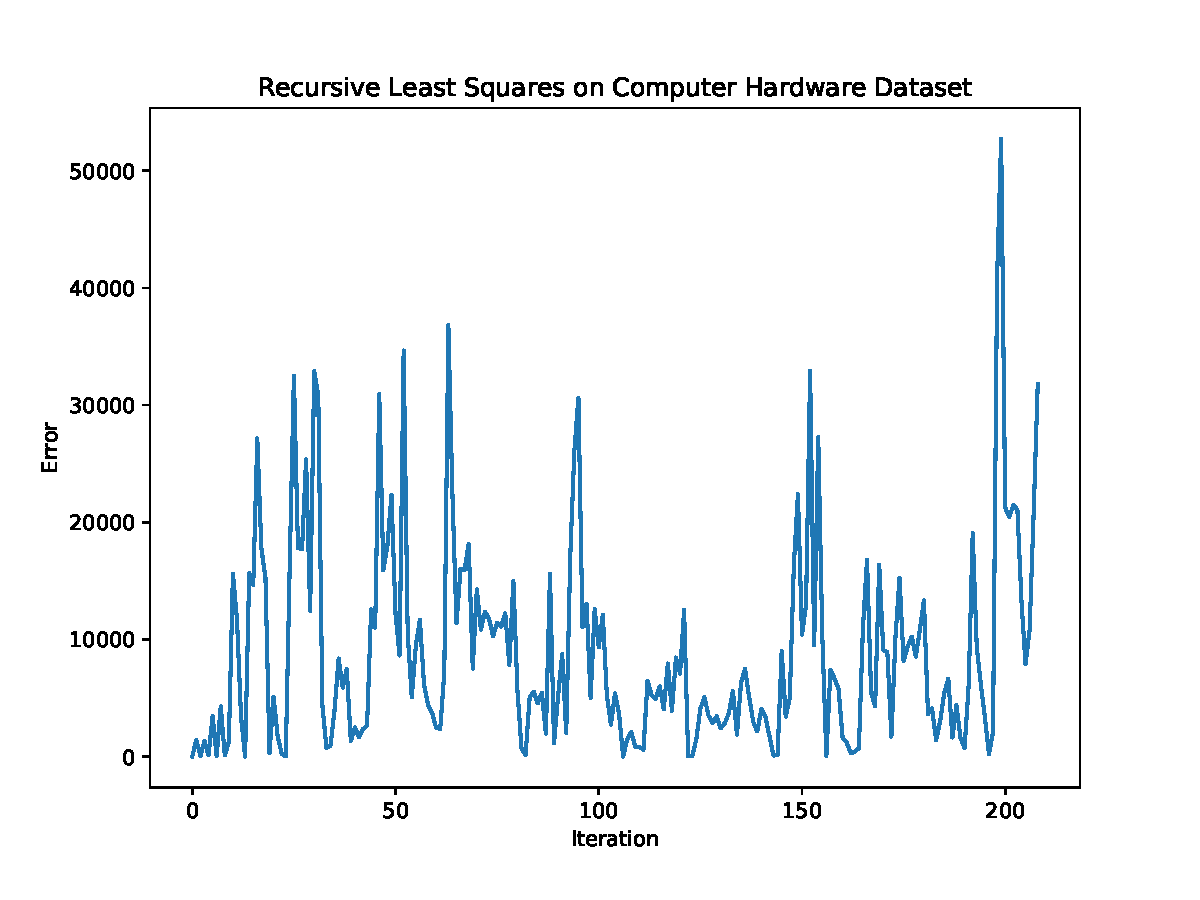
\includegraphics[width=0.33\textwidth]{Figures/uci_rls_iterError.pdf}}
    \subfloat[RLS with Padasip]{\label{fig:uci_pa}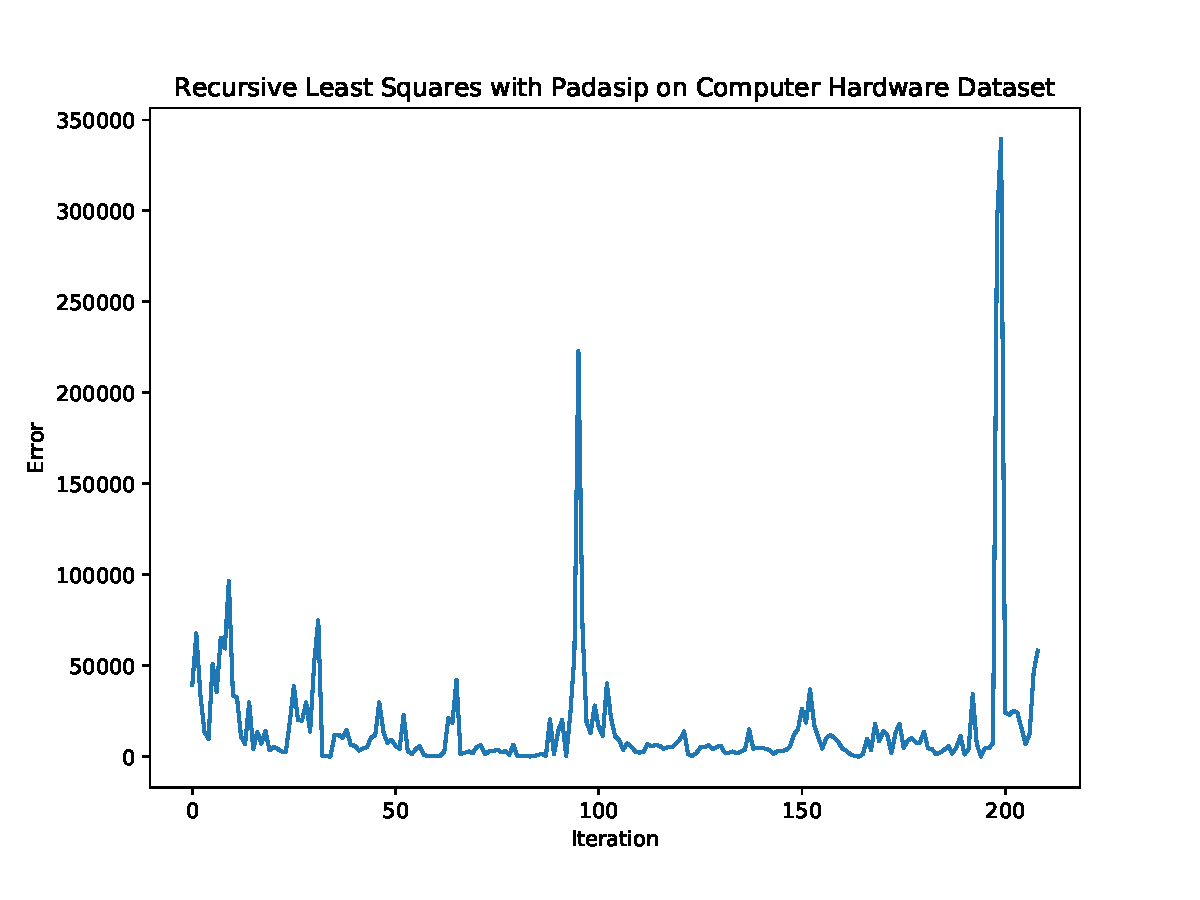
\includegraphics[width=0.33\textwidth]{Figures/uci_pa_iterError.pdf}}
    \caption{Linear Regression on Computer Hardware Dataset.}
    \label{fig:uci}
\end{figure}

\begin{table}[h!]
    \centering
    \caption{Table of correlation against ground truth on Computer Hardware Dataset.}
    \label{tab:task3_corr}
    \begin{tabular}{lrr}
    \toprule
    {} &         y &  w \\
    \midrule
    Ground Truth &  1.000000 &       NaN \\
    Closed Form  &  0.929995 &  1.000000 \\
    SGD          &  0.927807 &  0.974922 \\
    RLS          &  0.891165 &  0.740187 \\
    RLS Padasip  &  0.906713 &  0.733201 \\
    \bottomrule
    \end{tabular}
\end{table}


\section{Task 4}

\cref{fig:uci} shows the training plot for RLS implemented by myself and using the Python library, Padasip with the same exact parameters. Although the plots look dissimilar, \cref{tab:task3_corr} shows very similar predicted target and weights between both implementations. In addition, although the estimated weights for both RLS implementations do not correlate well with the closed form weights, it still produces similar performance the target compared to the closed form and SGD solutions.

It is discovered that the predicted results are very sensitive to the forgetting factor $\lambda$. A small tweak of $\lambda$, for example from 0.98 to 0.99 will significantly change the training plot and the predicted target and weights. Therefore, $\lambda$ needs to be tuned very well for different problems to be able to obtain good results.

\printbibliography

\end{document}